\documentclass{article}

\usepackage[english]{babel}
\usepackage[margin=3cm]{geometry}
\usepackage{graphicx}
\usepackage{float}
\usepackage{caption}
\usepackage{hyperref}
\usepackage{amsmath}
\usepackage{wrapfig}
\usepackage[parfill]{parskip}

% fonts
\usepackage[T1]{fontenc}
\usepackage{helvet}
\renewcommand{\familydefault}{\sfdefault}

\graphicspath{{img/}}

% theorem environment
\usepackage{amssymb}

\newtheorem{theorem}{Definition}[section]

\usepackage{enumitem}

\newenvironment{thmenum}
 {\begin{enumerate}[label=\upshape\bfseries(\roman*)]}
 {\end{enumerate}}


% code
\usepackage{minted}
\setminted{frame=single,framesep=3pt,linenos}
\usepackage{upquote}
\usepackage{color}

\begin{document}

\begin{titlepage}
    \author{Tuur Vanhoutte}
    \title{Advanced AI}
\end{titlepage}

\pagenumbering{gobble}
\maketitle
\newpage
\tableofcontents
\newpage

\pagenumbering{arabic}

\section{Reinforcement learning in context}

\begin{figure}[H]
    \centering
    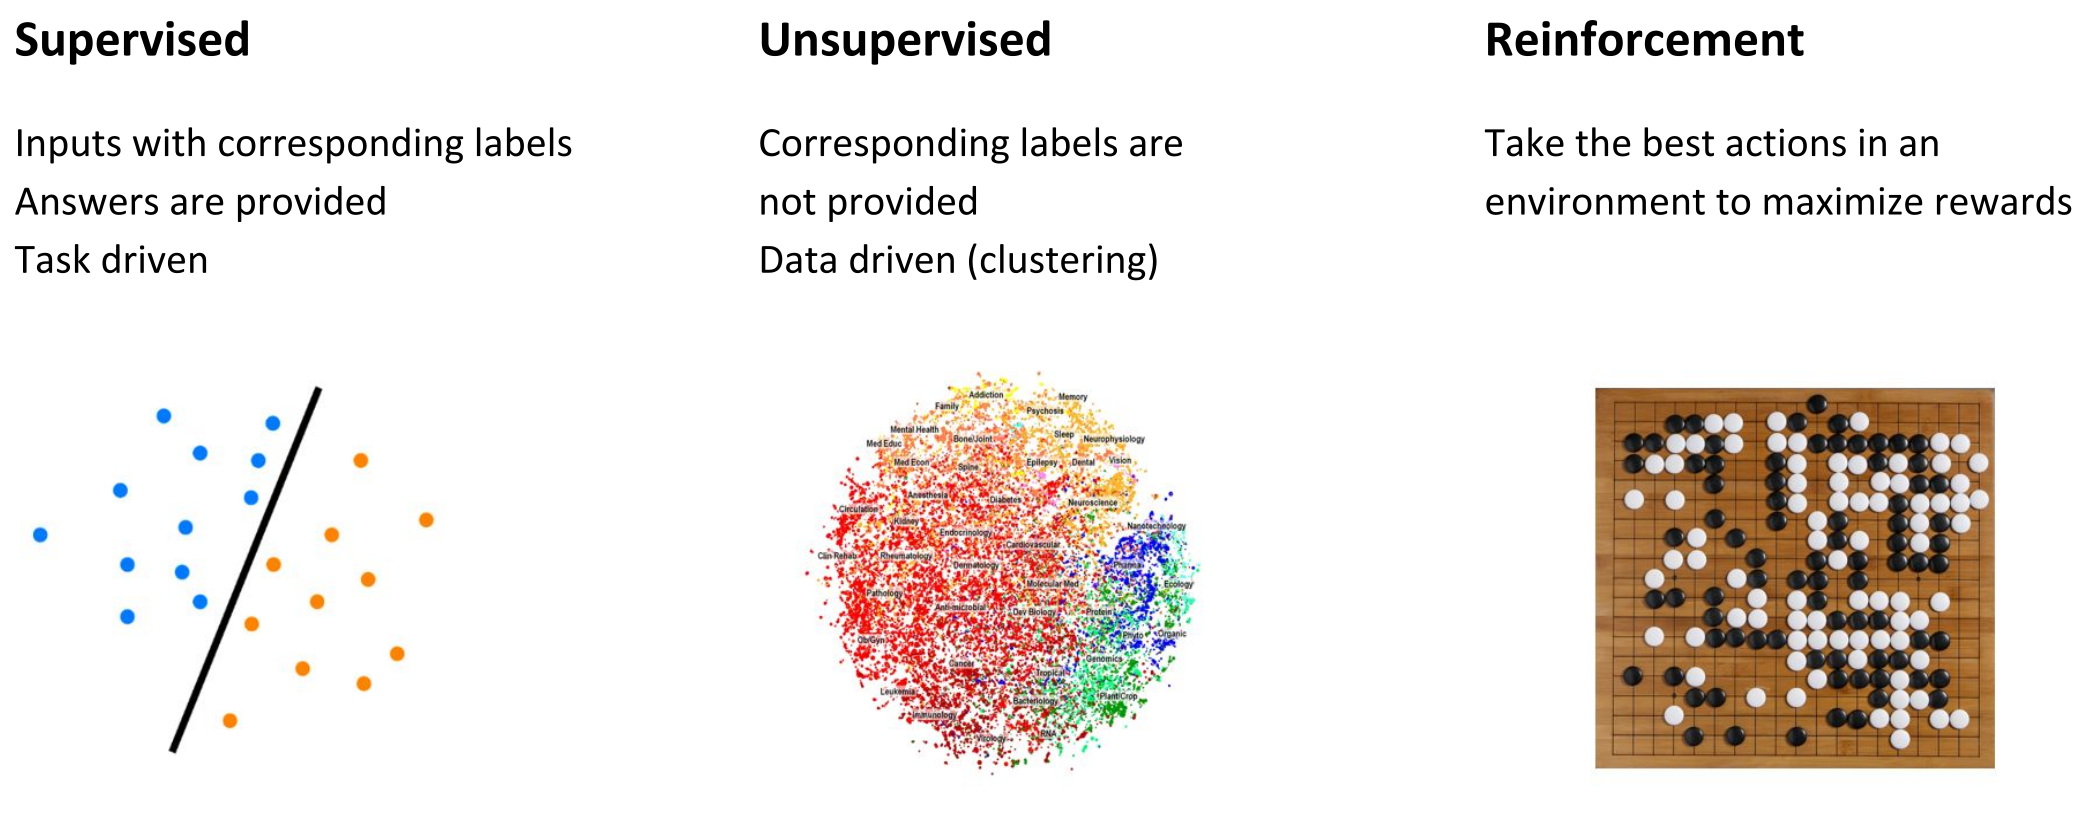
\includegraphics[width=0.8\textwidth]{img/leeralgoritmes.png}
    \caption{Overview learning algorithms}
\end{figure}


\subsection{What is Reinforcement Learning}

\begin{figure}[H]
    \centering
    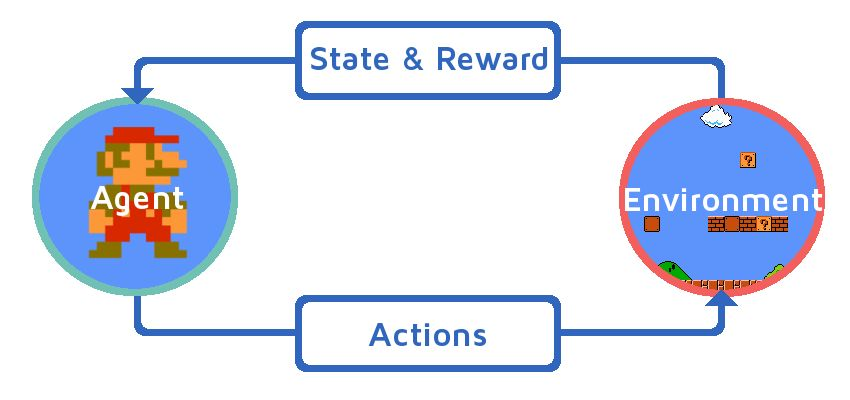
\includegraphics[width=0.5\textwidth]{img/reinforcement-learning-mario.png}
    \caption{An agent interacts with the environment, changes its state, and gets rewards}
\end{figure}

\subsubsection{Examples}

\begin{itemize}
    \item \url{http://www.youtube.com/watch?v=vZ7eHwVhe9c}
    \item \url{https://deepmind.com/blog/article/alphago-zero-starting-scratch}
    \item \url{https://www.youtube.com/watch?v=4MlZncshy1Q}
    \item \url{https://www.youtube.com/watch?v=eG1Ed8PTJ18}
    \item \url{http://www.youtube.com/watch?v=tlOIHko8ySg}
    \item \url{https://www.youtube.com/watch?v=W_gxLKSsSIE}
    \item \url{https://www.youtube.com/watch?v=ZBFwe1gF0FU}
    \item \url{https://www.youtube.com/watch?v=VCdxqn0fcnE}
    \item \url{https://www.youtube.com/watch?v=opsmd5yuBF0}
    \item \url{https://www.youtube.com/watch?v=gn4nRCC9TwQ}
    \item \url{http://www.youtube.com/watch?v=2cjkKnAxCug}
    \item \url{http://www.youtube.com/watch?v=kopoLzvh5jY}
\end{itemize}

\subsubsection{Reinforcement learning vs Deep learning}

\begin{theorem}
    \textbf{Deep learning} seeks to iteratively minimize a certain loss function 
    that indicates how accurate the functional representation of a system is.

    It responds to \textbf{patterns} in the data. It typically assumes the data
    it works with is \textbf{independent and identically distributed (IDD)}, and
    with a \textbf{stationary distribution}
\end{theorem}

\begin{theorem}
    \textbf{Reinforcement learning} seeks to iteratively maximize a certain notion of a numerical reward obtained through
    continued interaction with its environment.

    It learns to make \textbf{sequential decisions}. There is no need for the data
    to have \textbf{IDD} properties. The agent \textbf{can deal with non-stationarity} in 
    its environment during interaction
\end{theorem}

\begin{figure}[H]
    \centering
    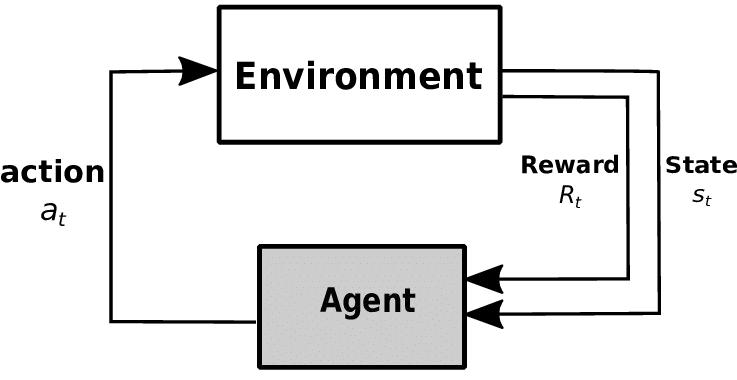
\includegraphics[width=0.5\textwidth]{img/rl-terminologies.png}
    \caption{Reinforcement Learning terminologies}
\end{figure}

\begin{theorem}[Agent]
    The learner and decision maker
\end{theorem}

\begin{theorem}[Environment]
    Where the agent learns and decides what actions to take
\end{theorem}

\begin{theorem}[Action]
    A set of actions which the agent can perform
\end{theorem}

\begin{theorem}[State]
    How the agent perceives the environment
\end{theorem}

\begin{theorem}[Reward]
    For each action selected by the agent, the environment provides a reward.
    Usually a scalar value.
\end{theorem}


\begin{figure}[H]
    \centering
    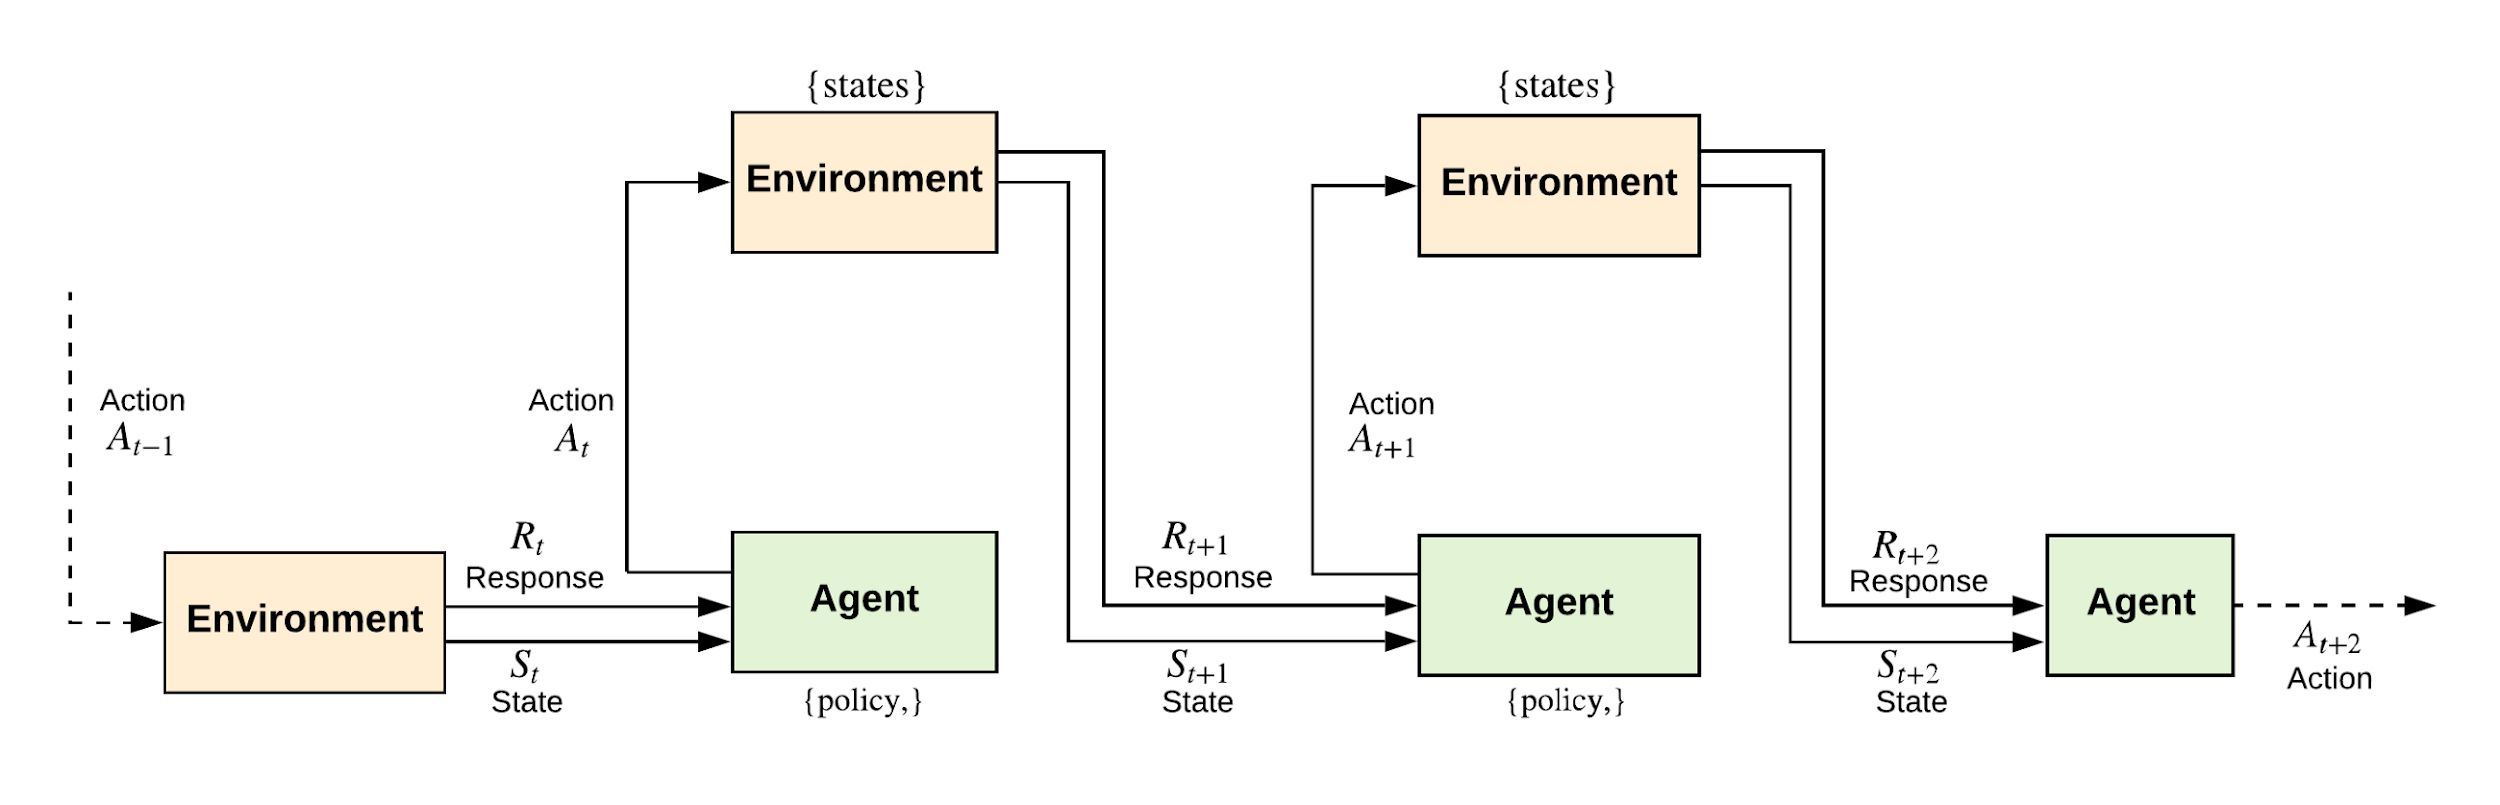
\includegraphics[width=0.8\textwidth]{img/rl-terminologies2.png}
    \caption{Reinforcement Learning terminologies}
\end{figure}

\begin{enumerate}
    \item The agent executes an action in the environment
    \item The environment responds with a reward and updates the state
    \item The agent decides the best action based on the new state and the reward it received
    \item Repeat \dots
\end{enumerate}

\begin{theorem}[Policy]
    The decision-making function (control strategy) of the agent, which represents
    a mapping from situations to actions. `Brain of the agent', the strategy your agent will follow.
\end{theorem}

\begin{theorem}[Value function]
    Mapping from states to real numbers, where the value of a state represents
    the long-term reward achieved starting from that state, and executing a particular
    policy.
\end{theorem}

\begin{theorem}[Function approximator]
    Refers to inducing a function from training examples. Standard 
    approximators include decision trees, neural networks, 
    and nearest-neighbor methods
\end{theorem}

\begin{theorem}[Markov Decision Process (MDP)]
    A probabilistic model of a sequential decision problem, where
    states can be perceived exactly, and the current state and action selected determine a
    probability distribution on future states. Essentially, the outcome of applying an action to a
    state depends only on the current action and state (and not on preceding actions or states).
\end{theorem}

\begin{theorem}[Model]
    The agent's view of the environment, which maps state-action pairs to probability
    distributions over states. Note that not every reinforcement learning agent uses a model of its
    environment
\end{theorem}

\subsection{Reinforcement learning taxonomy}

\begin{figure}[H]
    \centering
    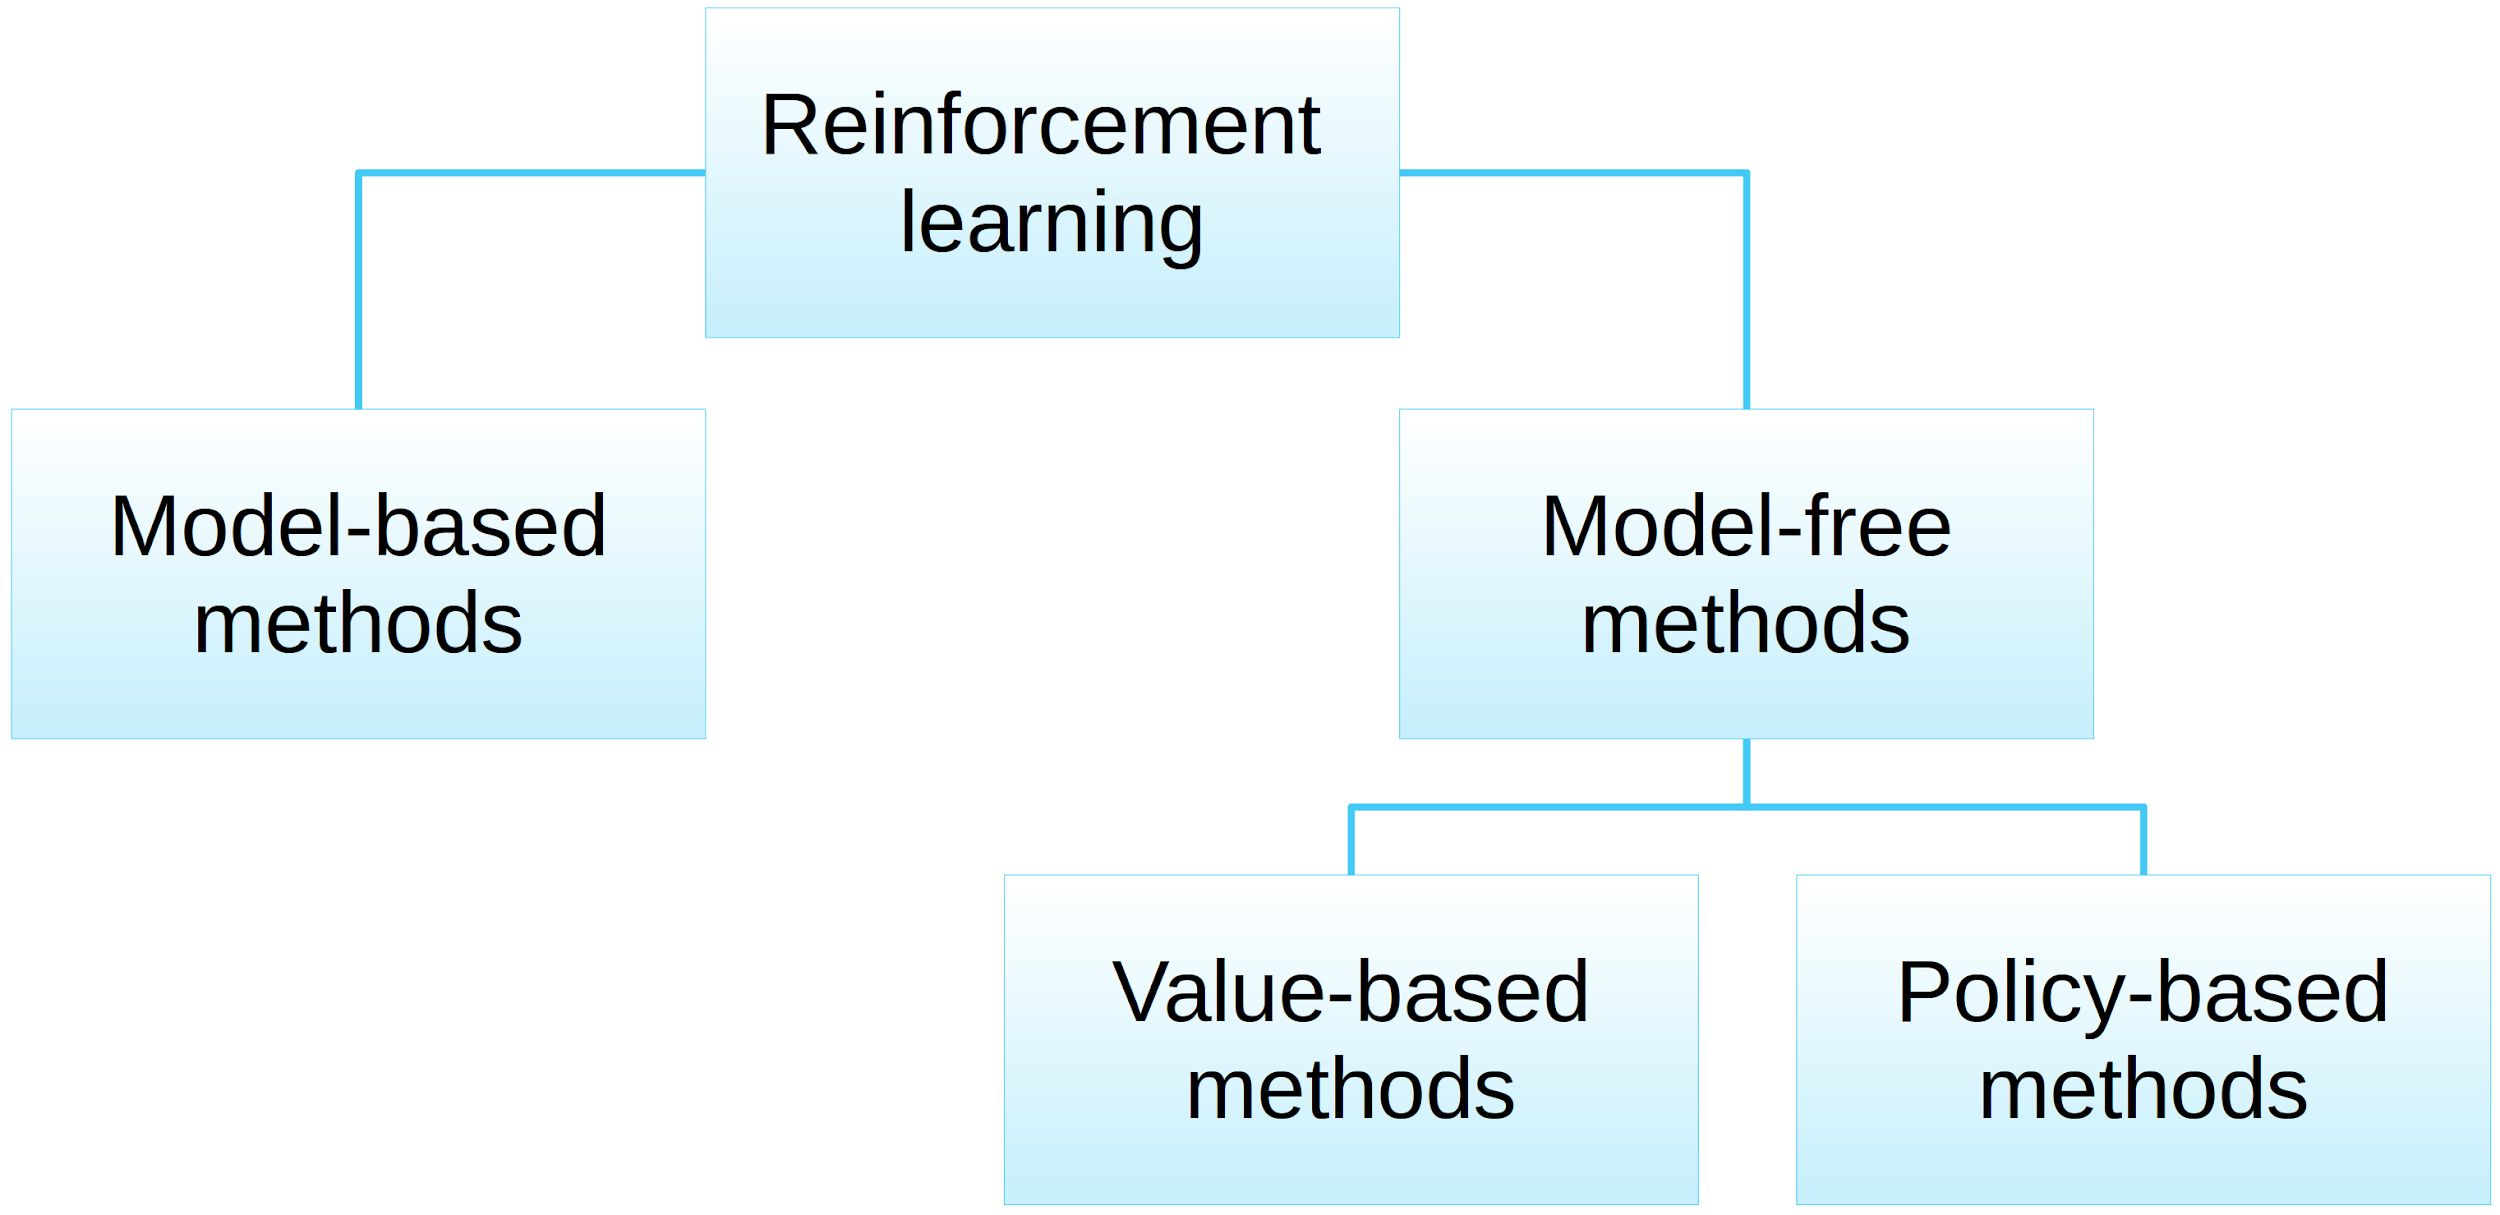
\includegraphics[width=0.5\textwidth]{img/rl-taxonomy.png}
    \caption{Two RL categories: model-based methods \& model-free methods}
\end{figure}

\subsubsection{Model based methods}

\begin{itemize}
    \item We can (partly) calculate the optimal actions using the model directly.
    \item The model may be known or learned.
    \item Can train from simulated experiences.
    \item Model-based RL has a strong advantage of being sample efficient.
    \item Usually computationally more complex.
    \item We will \textbf{not} focus on these methods in detail
\end{itemize}

\url{https://medium.com/@jonathan_hui/rl-model-based-reinforcement-learning-3c2b6f0aa323}

\subsubsection{Model-free}

\begin{itemize}
    \item The model is (partly) ignored.
    \item Needs no accurate representation of the environment in order to be effective.
    \item Computationally less complex.
    \item Actual experiences need to be gathered in order for training, which makes exploration more dangerous.
    \item Cannot carry an explicit plan of how environmental dynamics affects the system
\end{itemize}

\begin{figure}[H]
    \centering
    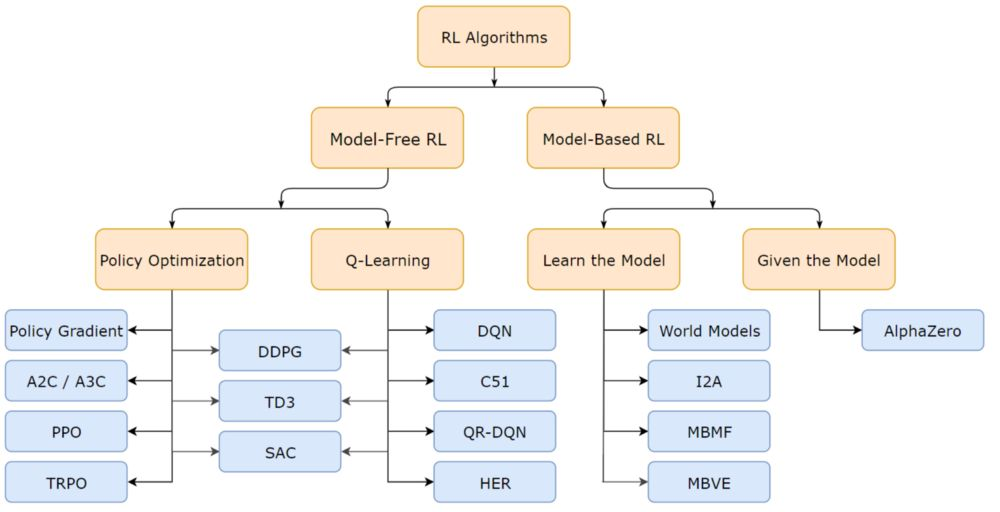
\includegraphics[width=0.5\textwidth]{img/modelbased-vs-modelfree2.png}
    \caption{Model based vs model-free}
\end{figure}

\begin{figure}[H]
    \centering
    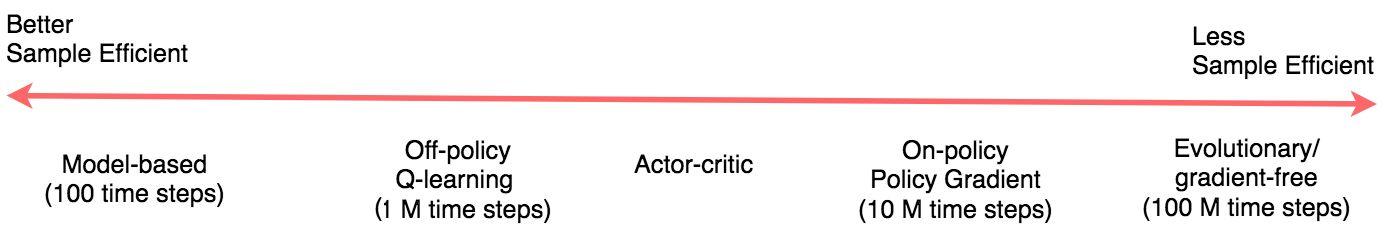
\includegraphics[width=0.75\textwidth]{img/modelbased-vs-modelfree.png}
    \caption{Model based vs model-free in terms of sample efficiency}
\end{figure}

\section{OpenAI Gym}

Gym is a toolkit for developing and comparing reinforcement learning algorithms. 
It supports teaching agents everything from walking to playing games like Pong or Pinball.

\begin{minted}{bash}
# installation
pip install gym
\end{minted}

Documentation: \url{https://gym.openai.com/docs/}

\end{document}